\section{Robótica de enjambre}
La robótica de enjambre consiste en el uso de robots relativamente sencillos que, al organizarse y funcionar en conjunto, pueden llevar a cabo tareas complejas que un solo robot no podría realizar \cite{robotica_enjambre2}. Esto proporciona soluciones flexibles, optimizadas y de un menor costo. Además, no se requiere un número específico de agentes robóticos ya que pueden ir desde las dos unidades hasta miles de ellas \cite{UNIDIRswarm}.

Algunas de las aplicaciones de la robótica de enjambre son el control de tráfico, realizar formaciones en movimiento, misiones de búsqueda y rescate, mapeo de entornos, simulación de comportamientos biológicos, exploración de zonas y comunicación de rutas. 

Estas últimas dos han sido estudiadas a profundidad para su implementación en la cosecha de la fresa donde el enjambre realiza la exploración de una zona de cultivo, analiza el estado de los frutos por medio de imágenes computacionales para determinar el momento óptimo para su cosecha y comunica los datos procesados para realizar una cosecha automatizada \cite{EnjambresCultivos}.

\subsection{Robótica de enjambre inspirada en peces}
En 2021 un equipo de investigadores del instituto Wyss de Harvard y la Escuela de Ingeniería y Ciencias Aplicadas John A. Paulson (SEAS) desarrollaron un robot llamado Bluebot inspirado en un pez. Este cuenta con dos cámaras y tres luces LED para su sistema de visión guiado. 

Los investigadores simularon una misión de búsqueda con una luz roja intermitente e implementaron un algoritmo de dispersión. Para iniciar, los Bluebots se dispersaron en el tanque y una vez que un robot detectó la luz roja, sus leds comenzaron a parpadear, lo que activó el algoritmo de agregación al resto de robots que lograron sincronizar sus movimientos y agruparse al rededor del robot que detectó la luz, imitando a un banco de peces real \cite{Bluebot}.

\begin{figure}[H]
	\centering
	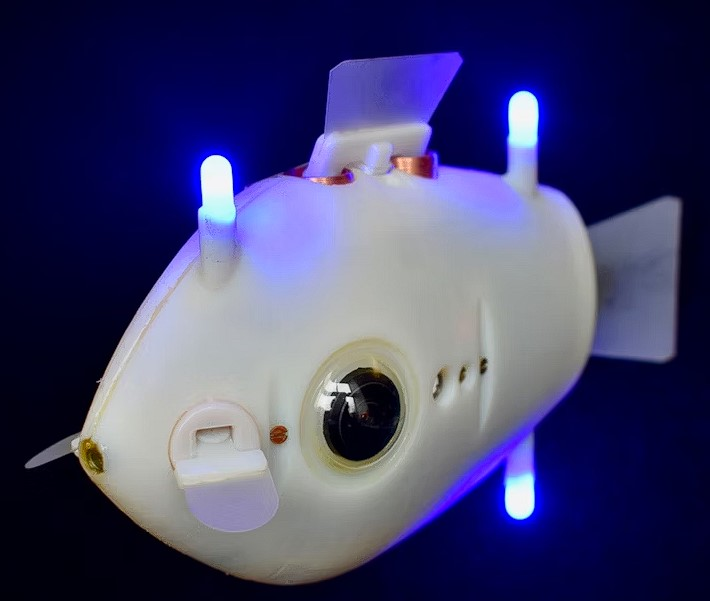
\includegraphics[width=0.5\textwidth]{Bluebot.jpg}
	\caption{Prototipo físico de Bluebot\cite{Bluebot}.}
	\label{fig:bluebot}
\end{figure}

\section{Robotarium de Georgia Tech}
En el Instituto Tecnológico de Georgia se ha desarrollado el proyecto Robotarium \cite{Robotarium}. Se realizó para proveer acceso gratuito a una plataforma de robótica de enjambre a la que pueda acceder cualquier persona del mundo. Lo único que se necesita para experimentar con la plataforma es descargar un simulador en Matlab o Python, registrarse en la página de Robotarium y esperar la aprobación por parte de un administrador para realizar el experimento.

\begin{figure}[H]
	\centering
	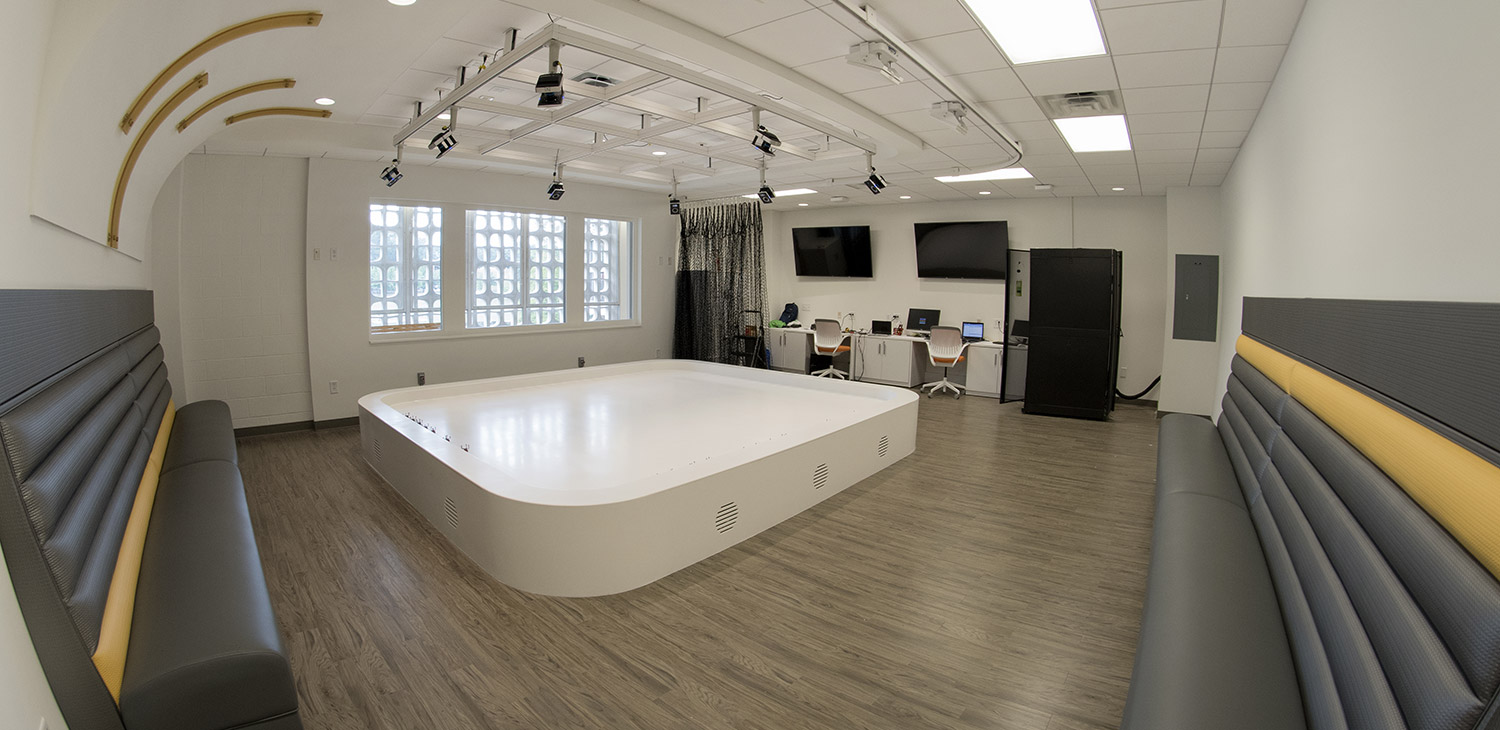
\includegraphics[width=0.5\textwidth]{robotarium.jpg}
	\caption{Laboratorio Robotarium de Georgia Tech \cite{Robotarium}.}
	\label{fig:robotarium}
\end{figure}

\section{Robotat de la Universidad del Valle de Guatemala}
En el Centro de Innovación y Tecnología de la Universidad del Valle de Guatemala, se encuentra una plataforma de robótica para experimentación llamada Robotat la cual está inspirada en el Robotarium del Instituto Tecnológico de Georgia. Esta se conforma de una plataforma de acero y plycem con un espacio útil de 5 $\times$ 5 $\times$ 3 m, capaz de soportar cargas puntuales de hasta dos toneladas. También cuenta con un sistema de captura de movimiento de OptiTrack, compuesto de seis cámaras Prime$^x$ 41 de alta precisión y baja latencia para realizar experimentos en tiempo real. Además, el sistema funciona con una red local inalámbrica WiFi a través de la cual se realiza la comunicación entre robots \cite{Robotat}. 

Para el funcionamiento del sistema OptiTrack, se utilizan ``marcadores'' que son figuras plásticas con reflectivos. Estos permiten reflejar la luz infrarroja que emiten las cámaras para obtener, de manera precisa, la posición y el movimiento de objetos en un espacio tridimensional.

\begin{figure}[H]
	\centering
	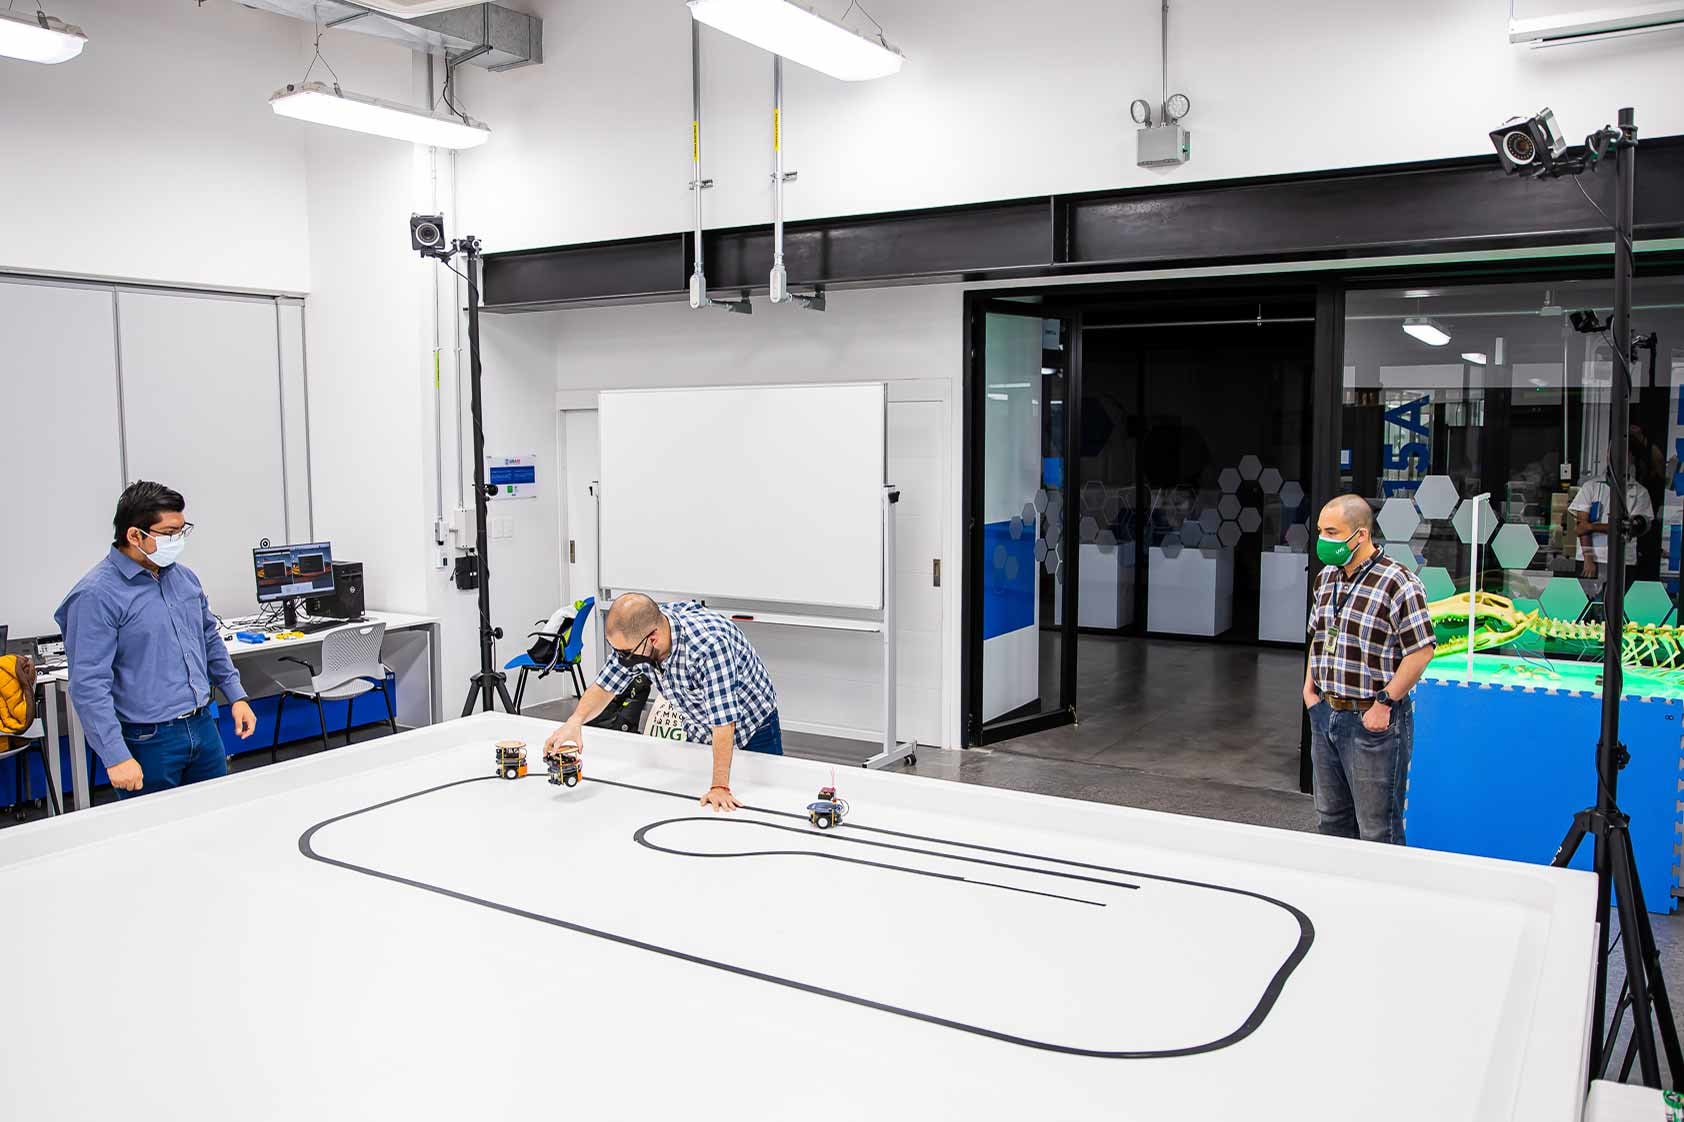
\includegraphics[width=0.5\textwidth]{robotatUVG.jpg}
	\caption{Plataforma Robotat de la Universidad del Valle de Guatemala \cite{imgRobotat}.}
	\label{fig:robotat}
\end{figure}

\section{Trabajos previos de robótica de enjambre en la UVG}
A continuación se presentan algunos de los trabajos realizados en el área de robótica de enjambre.

\subsection{Validación de algoritmos de algoritmos de \textit{Particle Swarm Optimization} (PSO) y \textit{Ant Colony Optimization} (ACO)}
La tesis de Jonathan Menéndez \cite{MenendezJ_2023_tesis} se enfocó en realizar pruebas físicas para validar los algoritmos de robótica de enjambre PSO y ACO utilizando los robots móviles Pololu 3pi+ en la plataforma de Robotat. 

Luego de realizar múltiples pruebas físicas, se encontró que el algoritmo de ACO es capaz de generar trayectorias de manera satisfactoria en el ecosistema del Robotat, respetando las limitaciones físicas de espacio en la mesa para no colisionar y evitar que las cámaras de OptiTrack pierdan la detección de los agentes. Además, este algoritmo demostró tener una mayor eficiencia al corregir las diferencias entre el nodo de inicio y la posición inicial del robot al orientarlo hacia el punto de inicio. 

Dichos estudios se limitaron al espacio disponible en la mesa de la plataforma del Robotat, a un espacio libre de obstáculos y a la implementación de solo diez Pololu 3pi+ debido a la disponibilidad de equipo. 

\subsection{Algoritmo de sincronización y control de sistemas de robots multiagente para misiones de búsqueda}
El trabajo de investigación de Andrea Maybell Peña \cite{PenaAM_2019_tesis} se basó en utilizar un sistema de robots multi-agente para realizar misiones de búsqueda. El algoritmo se basa en la teoría de grafos y el control moderno para tener formaciones específicas de los agentes que permiten su movilización a través de obstáculos que se limitaron a una geometría toroidal y la cantidad de agentes robóticos se limitó a diez unidades del modelo E-Puck de GCtronic.

Se realizó la implementación del algoritmo en el simulador Webots de Cyberbotics. Como resultado se obtuvo una tasa de éxito del 80\% utilizando el algoritmo completo para llegar a la meta.

\begin{figure}[H]
	\centering
	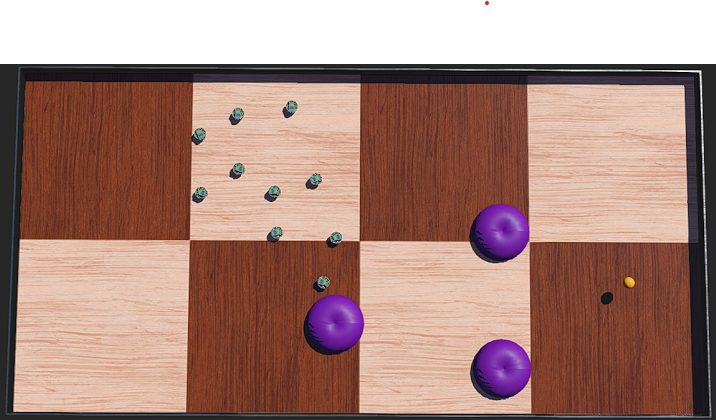
\includegraphics[width=0.4\textwidth]{simulacion_inicio_tesis_andreaPena.png} 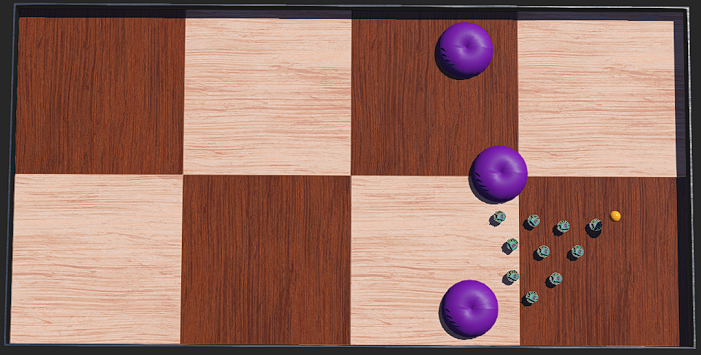
\includegraphics[width=0.4\textwidth]{simulacion_final_tesis_andreaPena.png}
	\caption{Simulación en Webots implementando el algoritmo para evadir obstáculos \cite{imgRobotat}.}
	\label{fig:tesis_andreaPena}
\end{figure}

\subsection{Validación de un algoritmo de inteligencia de enjambre enfocado en sincronización y control de formaciones de sistemas robóticos multi-agente en un entorno físico}
En el trabajo de investigación de Alejandro Rodríguez \cite{RodriguezJA_2023_tesis}se realizó una validación del algoritmo de inteligencia de enjambre enfocado a sincronización vertical y control de formaciones de sistemas robóticos multi-agente. La validación se realizó utilizando el ecosistema del Robotat de la Universidad del Valle de Guatemala y los robots Pololu 3pi+ modificados.

Para la validación física, se realizaron diversos experimentos donde se evaluó el desempeño de cada agente, la generación de trayectorias, el posicionamiento de los agentes, las distintas configuraciones de formación y los escenarios utilizando obstáculos.

Los experimentos realizados se limitaron a utilizar un máximo de nueve agentes robóticos debido a su disponibilidad en la universidad, el tiempo máximo por semana para realizar pruebas en el Robotat fue de seis horas y estas se realizaron utilizando obstáculos estáticos.

Los resultados de la experimentación demostraron que, el algoritmo evade los obstáculos satisfactoriamente y mantiene una distancia adecuada entre agentes. Sin embargo, el algoritmo en simulación es aproximadamente un 70\% más rápido que en físico. Esto se debe a que cada prueba física tomaba al rededor de 8 minutos debido a la latencia del servidor que aumentaba con el número de agentes conectados. 


